%%%%%%%%% PROJECT DESCRIPTION  -- 15 pages (including Prior NSF Support)

\required{Project Description}
\begin{center}
%\emph{Maximum of 15 pages}
\end{center}
%The Project Description (including Results from Prior NSF Support, which is
%limited to five pages) may not exceed 15 pages. Visual materials, including charts,
%graphs, maps, photographs and other pictorial presentations are included in the
%15-page limitation. PIs be cautioned that the project description must
%be self-contained and that URLs that provide information related to the proposal
%should not be used. \\
%
%All proposals to NSF are reviewed utilizing the two merit review criteria,
%intellectual merit and broader impacts. \\
%
% The Project Description should provide a clear statement of the work 
% to be undertaken and must include: objectives for the period of the proposed 
% work and expected significance; relation to longer-term goals of the PI's 
% project; and relation to the present state of knowledge in the field, 
% to work in progress by the PI under other support and to work in progress 
% elsewhere.

%%%%%%%%%%%%%%%%%%%%%%%%%%%%%%%%%%%%%%%%%%%%%%%%%%%%%%%%%%%%%%%%%%%%%%
%INTRO
%%%%%%%%%%%%%%%%%%%%%%%%%%%%%%%%%%%%%%%%%%%%%%%%%%%%%%%%%%%%%%%%%%%%%%
\section*{Introduction}

While the potential roles of hybridization and introgression as agents of evolution have long been appreciated \citep{Anderson1948, Anderson1954, Stebbins1959}, only recently have technological innovations allowed for characterization on a genome-wide scale. Multiple genome-wide studies have now reported substantial inter-taxon introgression in both plant \citep{Hufford2013, renaut2013} and animal \citep{consortiumbutterfly2012, staubach2012} species. Introgression has been found across substantial portions of genomes and specifically at loci thought to underlie adaptation. 

In the investigation proposed here, we will build upon our previous work in maize (\emph{Zea mays} ssp. \emph{mays}) and its wild relatives (\emph{Zea} spp.; collectively referred to as teosinte) in order to characterize the evolutionary role of hybridization and introgression in the genus \emph{Zea}. This study system is ideally suited for such research due to its well-characterized history, large natural populations, and the availability of exceptional genomic resources \citep{Hufford2012}. The history of \emph{Zea} allows us to assess the genome-wide effects of hybridization and introgression at two different timescales: 1) A more evolutionary timescale spanning 60,000 generations of divergence amidst gene flow between the subspecies \emph{Zea mays} ssp. \emph{parviglumis} and \emph{Zea mays} ssp. \emph{mexicana}; and 2) An ecological timescale ($\sim$3000-9,000 generations) in which maize has spread across the Americas and adapted to local conditions, potentially through hybridization and introgression from endemic wild relatives that are allopatric to the progenitor of maize. Our analysis on an evolutionary timescale will generate basic knowledge of the process of incipient speciation and the porous nature of genomes of diverging species, whereas our analysis on an ecological timescale can inform, for example, the study of biological invasions if maize is viewed as an invasive species aided in colonization by gene flow from locally-adapted native species.

%%%%%%%%%%%%%%%%%%%%%%%%%%%%%%%%%%%%%%%%%%%%%%%%%%%%%%%%%%%%%%%%%%%%%%
%OBJECTIVES
%%%%%%%%%%%%%%%%%%%%%%%%%%%%%%%%%%%%%%%%%%%%%%%%%%%%%%%%%%%%%%%%%%%%%%
\section*{Objectives}
	
We will leverage the resources of the \emph{Zea} study system to address two primary objectives:

\subsection*{Objective I: Hybrid Zones: Assess the evolutionary significance of hybridization and introgression in locally-adapted, parapatric wild \emph{Zea} taxa}
\emph{Zea mays} ssp. \emph{parviglumis} (the wild progenitor of maize; hereafter, \emph{parviglumis}) and \emph{Zea mays} ssp. \emph{mexicana} (hereafter, \emph{mexicana}) diverged approximately 60,000 BP \citep{Ross-Ibarra2009a} and have parapatric distributions: while \emph{parviglumis} occurs in the warm lowlands of southwest Mexico, \emph{mexicana} is found in the cool highlands of the Mexican Central Plateau. Narrow regions of substantial admixture between these wild subspecies have been discovered at middle elevations \citep{Fukunaga2005, Pyhajarvi2013}. Through targeted collections, generation of high-density genotyping data, population genomic analyses, and common garden experiments, we will address the following research questions and work toward establishing this system as a model for the study of hybrid zones:
\begin{adjustwidth}{5em}{5em}
\subsubsection*{\emph{Research Question IA) What fraction of the genome is porous to gene flow in hybrid zones?}}

\subsubsection*{\emph{Research Question IB) How does the fitness of \emph{parviglumis}, \emph{mexicana}, and hybrid populations vary across the hybrid zone?}}

\subsubsection*{\emph{Research Question IC) Are allele frequency clines at loci associated with fitness traits in \emph{mexicana} and \emph{parviglumis} steeper than those at non-associated loci?}}
\end{adjustwidth}
\vspace{0.5cm}

\subsection*{Objective II: Genus-wide Introgression: Determine the extent to which hybridization and introgression have altered the \emph{Zea} genus during the post domestication spread of maize}
Maize was domesticated in southwest Mexico from \emph{parviglumis} $\sim$9,000 BP \citep{Matsuoka2002} and quickly spread throughout North America, bringing this crop into sympatry with new species of teosinte \citep{Vigouroux2008a}. Through a combination of dense genotyping of range-wide samples of maize and teosinte and targeted, full-genome sequencing, we will assess three questions regarding the importance of introgression during the spread of maize:
\begin{adjustwidth}{5em}{5em}	
\subsubsection*{\emph{Research Question IIA) Was the spread of maize facilitated by gene flow from locally-adapted wild \emph{Zea}?}}
\subsubsection*{\emph{Research Question IIB) What is the geographic scale of adaptive introgression?}}
\subsubsection*{\emph{Research Question IIC) Did maize serve as a bridge for gene flow between previously isolated \emph{Zea} taxa?}}
\end{adjustwidth}
\vspace{0.5cm}

%%%%%%%%%%%%%%%%%%%%%%%%%%%%%%%%%%%%%%%%%%%%%%%%%%%%%%%%%%%%%%%%%%%%%%
%RATIONALE AND SIGNIFICANCE
%%%%%%%%%%%%%%%%%%%%%%%%%%%%%%%%%%%%%%%%%%%%%%%%%%%%%%%%%%%%%%%%%%%%%%
\section*{Rationale and Significance}
Pioneers in evolutionary biology including G. Ledyard Stebbins and Edgar Anderson recognized the important role hybridization and introgression could play in adaptation and speciation \citep{Anderson1948, Anderson1954}. These evolutionary forces were thought to be particularly influential when environmental conditions encountered by a species were marginal, variable, or new \citep{Stebbins1959}. More recently, theoretical and empirical investigations of hybridization have focused on hybrid zones, defined as regions where distinct taxa co-occur and mate, resulting in progeny of mixed ancestry \citep{HarrisonHybridZone}. 

While hybrid zone theory has progressed and many compelling empirical examples have been identified based on hybrid morphology and limited genetic data \citep{Delmore2013, Galindo2013, Parchman2013, Smith2013a}, several outstanding questions remain. Additional study is needed to determine whether hybrid zones are primarily maintained as tension zones in which hybrids are selected against or as ecotones where hybrids have an advantage under certain environmental conditions \citep{Kruuk1999, Rasmussen2012, Smith2013b}. Moreover, genome-wide analysis of the fraction of the genome that is porous to gene flow in hybrid zones is rare and will likely offer considerable insight.  For example, vanguard genomic studies of hybridization and introgression suggest that rates of gene flow vary substantially across loci and that chromosomal rearrangements (\emph{e.g.}, inversions and translocations) may restrict gene flow in hybridizing species \citep{Hufford2013, Barb2014, Poelstra2014, SoriaCarrasco2014}.
	 
Both wild and domesticated \emph{Zea} offer exciting opportunities to study hybridization. The subspecies \emph{parviglumis} and \emph{mexicana} are distributed across a steep altitudinal gradient and differ for traits that are thought to be adaptive in the highlands such as the presence of macrohairs and stem pigmentation.  Both of these traits are found in highland \emph{mexicana} but are lacking in lowland \emph{parviglumis}. Analysis of $\sim$100 microsatellite markers genotyped in a range-wide sample of \emph{parviglumis} and \emph{mexicana} has previously identified elevated admixture between the subspecies in two geographically-distinct, mid-elevation regions: eastern Jalisco state and the eastern Balsas River Basin \citep{Fukunaga2005}.  The positioning of these populations at intermediate locations between the known distributions of the two subspecies suggests they may represent stable zones of hybridization.

Our recent genome-wide analysis ($\sim$40,000 SNPs) of a population from the putative eastern Balsas hybrid zone revealed extensive subspecies admixture across all individuals sampled \citep{Pyhajarvi2013}.  Genotype data from this hybrid population were compared to those of non-admixed populations revealing relatively short shared haplotypes between these two groups, a result suggesting continual gene flow between \emph{parviglumis} and \emph{mexicana} at this hybrid zone over a substantial period of time \citep{Pyhajarvi2013}.  Longer shared haplotypes were found in the hybrid population in chromosomal regions identified as potential inversions based on high differentiation and linkage disequilibrium between \emph{parviglumis} and \emph{mexicana} \citep{Pyhajarvi2013}.  These regions may be particularly resistant to gene flow.  While these initial findings are suggestive of hybrid zone dynamics in teosinte, further population genomic investigation is necessary to compare the genomic architecture of hybridization and introgression both across populations within hybrid zones as well as between distinct hybrid zones.  Furthermore, evaluation of the fitness of \emph{parviglumis}, \emph{mexicana}, and hybrid samples in reciprocal transplants will shed light on whether hybridization of teosinte subspecies is sustained through tension zone or ecotone processes (see \textbf{Objective I}).

In addition to the ongoing hybridization between \emph{parviglumis} and \emph{mexicana} occurring since divergence $\sim$60,000 BP, gene flow between domesticated maize and various taxa of the genus \emph{Zea} has been detected based on both hybrid morphologies observed in the field \citep{wilkes1967teosinte, Wilkes1977} and genetic data \citep{Ross-Ibarra2009a}. Domestication of maize from \emph{parviglumis} occurred recently on an evolutionary timescale ($\sim$9,000BP; \citealt{Matsuoka2002}) and was followed by rapid spread of the crop across the Americas during the following millennia \citep{Piperno2001,Grobman2012}. During this diffusion maize was brought into sympatry with new wild relatives that were likely allopatric to the progenitor of maize (\emph{i.e., parviglumis}) for long periods prior to domestication \citep{hufford2012inferences}. 

Our recent work has provided evidence of introgression from \emph{mexicana} into maize during its earliest diffusions into the highlands of the Mexican Central Plateau.  Consistent introgression into maize was found in several highland maize populations at QTL for phenotypes (\emph{e.g.}, pigment and macrohairs) that distinguish highland \emph{mexicana} from lowland \emph{parviglumis} \citep{Hufford2013}. Our interpretation of this result is that maize received adaptive introgression from \emph{mexicana} that allowed the crop to spread into the highlands of Mexico. 

Subsequent to its diffusion into the Mexican highlands, maize spread into sympatry with additional teosinte taxa in Guatemala including \emph{Zea luxurians} (hereafter, \emph{luxurians}) and \emph{Zea mays} ssp. \emph{huehuetenangensis} (hereafter, \emph{huehuetenangensis}). Based on analysis of a small number of loci ($n=456$) \mbh{is this the number of SNPs in the 26 nuclear loci?}, \emph{mexicana} haplotypes have been found segregating in \emph{luxurians} \citep{Ross-Ibarra2009a}.  Since \emph{mexicana} and \emph{luxurians} are entirely allopatric in their distributions, this suggests maize has served as a bridge for gene flow between these two taxa.  Further work will be necessary to explore this possibility and to assess if maize has, more generally, altered the genomes of \emph{Zea} species through gene flow during its spread across the Americas.  Yet another fascinating question that remains to be answered is whether additional \emph{Zea} taxa, like \emph{mexicana}, have donated adaptive alleles to maize that allowed it to successfully colonize new habitats (see \textbf{Objective II}).

%%%%%%%%%%%%%%%%%%%%%%%%%%%%%%%%%%%%%%%%%%%%%%%%%%%%%%%%%%%%%%%%%%%%%%
%PRELIMINARY RESULTS
%%%%%%%%%%%%%%%%%%%%%%%%%%%%%%%%%%%%%%%%%%%%%%%%%%%%%%%%%%%%%%%%%%%%%%
\section*{Preliminary Results}

Our previous publications suggest \emph{Zea} is a promising model system for exploring the evolutionary role of hybridization and introgression (\emph{e.g.},  \citealt{Ross-Ibarra2009a, vanheerwaarden2011a, Hufford2013, Pyhajarvi2013}).  To further refine our research questions and provide preliminary results for this proposal we have analyzed a previously published data set \citep{vanheerwaarden2011a, Fang2012} of 983 SNPs genotyped across a panel of $>2,000$ samples including all subspecies and species of teosinte and an Americas-wide sample of maize landraces (\emph{i.e.}, ancient farmer varieties of maize).  While the low density of the markers in this data set precludes genome-wide inferences and haplotype-based analyses, the comprehensive taxon sampling makes this an ideal resource for guiding future research.

\subsection*{Evidence for hybrid zones between \emph{parviglumis} and \emph{mexicana}}

We have assessed evidence for admixture between \emph{parviglumis} and \emph{mexicana} using the range-wide sampling of hundreds of populations in the 983-SNP data set.  The probability of each sample's assignment to \emph{parviglumis} and \emph{mexicana} groups was calculated using the program STRUCTURE \citep{Pritchard2000} and individuals were sorted in order of increasing altitude.  We find that individuals from several mid-elevation populations show appreciable assignment to both \emph{parviglumis} and \emph{mexicana} groups (red underscored individuals in Figure \ref{fig:structure}) and likely represent hybrid populations.  

\begin{figure}
  \centering
   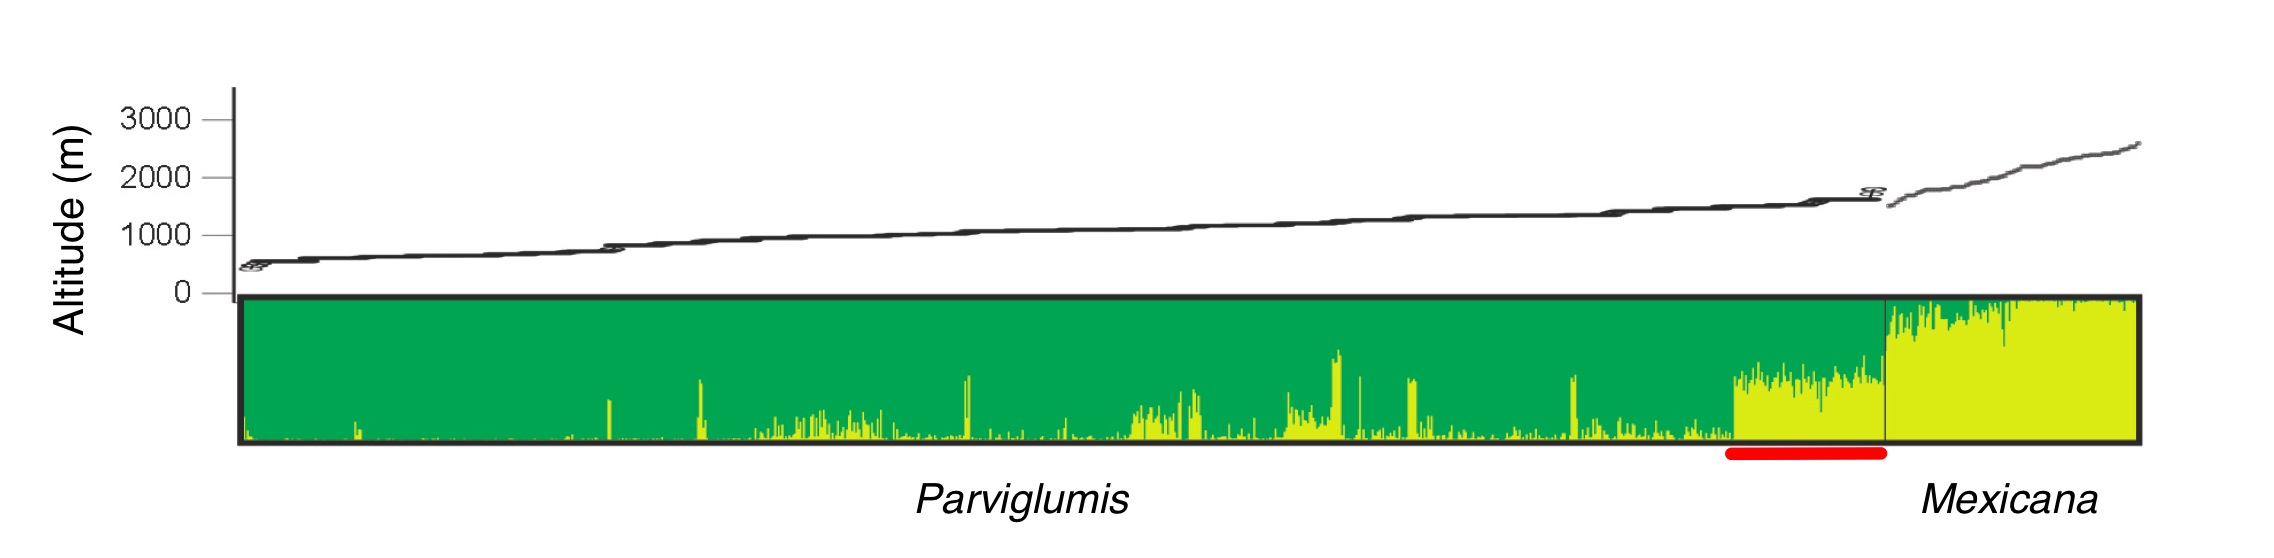
\includegraphics[width=0.95\textwidth]{structure.jpg}
    \caption{Assignment of \emph{parviglumis} and \emph{mexicana} individuals to K=2 groups using the Bayesian assignment algorithm of STRUCTURE \citep{Pritchard2000}.  Individuals are sorted by increasing altitude as indicated by the plot above the bar chart. Individuals from mid-elevation, hybrid zone populations are underscored in red.} 
\label{fig:structure}
\end{figure}

Several admixed populations cluster in two geographically distinct regions of Mexico: the eastern Balsas River Basin and eastern Jalisco state.  These locations fall at intermediate locations between the main distributions of \emph{parviglumis} and \emph{mexicana} (Panel A, Figure \ref{fig:pies}).  Hybrid populations from eastern Jalisco state are found at higher elevation (average elevation = 1632m) than hybrid populations in the eastern Balsas (average elevation = 1531m) and also show a higher proportion of membership in a \emph{mexicana} (\emph{i.e.}, highland teosinte) group (Panels B and C, Figure \ref{fig:pies}).  These findings suggest that hybrid populations from distinct environments may vary in proportion of ancestry from these two subspecies in a manner that is adaptive.  Estimates of pairwise population differentiation also suggest that hybrid populations in the Balsas and Jalisco are distinct in that Jalisco populations are less differentiated from \emph{mexicana} than hybrid populations in the Balsas (Table \ref{tab:Fst}).  Not surprisingly, populations in both hybrid zones are less differentiated from \emph{mexicana} and \emph{parviglumis} than these subspecies are from each other.

\begin{SCfigure}
  \centering
   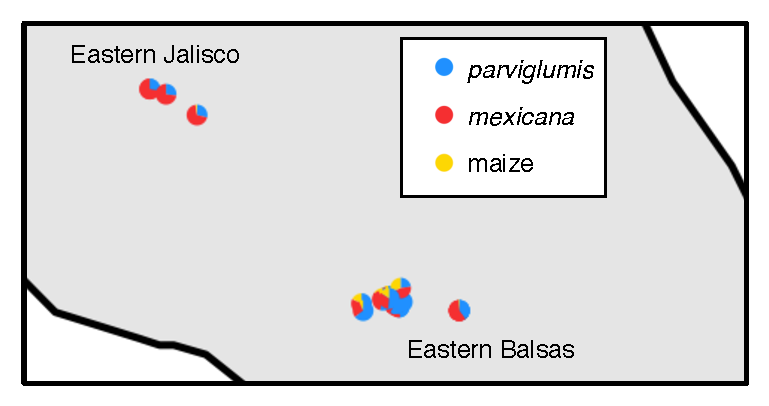
\includegraphics[width=0.6\textwidth]{pies.pdf}
    \caption{Proportion of assignment of hybrid populations to \emph{parviglumis}, \emph{mexicana}, and maize groups in putative Eastern Jalisco and Eastern Balsas hybrid zones} 
\label{fig:pies}
\end{SCfigure}

\begin{table}[]
\rowcolors{2}{gray!25}{white}
\begin{center}
\caption{Pairwise $F_{ST}$ between teosinte and hybrid populations} \label{tab:Fst}
\begin{tabular}{lcccc}\\\toprule
{\bf Taxon}&{\bf \emph{parviglumis}}&{\bf \emph{mexicana}}&{\bf Jalisco Hybrids}&{\bf Balsas Hybrids}\\\midrule
{\bf \emph{parviglumis}}&---&---&---&---\\
{\bf \emph{mexicana}}&0.107&---&---&---\\
{\bf Jalisco Hybrids}&0.059&0.064&---&---\\
{\bf Balsas Hybrids}&0.057&0.074&0.034&---\\\bottomrule
\end{tabular}
\end{center}
\end{table} 

\subsection*{Evidence for hybridization across the genus \emph{Zea}}

TreeMix Results\\

ILS Results\\

Chr4 Inversion Results?\\

%%%%%%%%%%%%%%%%%%%%%%%%%%%%%%%%%%%%%%%%%%%%%%%%%%%%%%%%%%%%%%%%%%%%%%
%SPECIFIC OBJECTIVES
%%%%%%%%%%%%%%%%%%%%%%%%%%%%%%%%%%%%%%%%%%%%%%%%%%%%%%%%%%%%%%%%%%%%%%
\section*{Research Plan}

\subsection*{Objective I: Hybrid Zones}

\subsubsection*{Research Question IA) What fraction of the genome is porous to gene flow in hybrid zones?}

Currently, very few studies have dissected the genome-wide architecture of hybridization and introgression in a hybrid zone (but see \citealt{staubach2012}). Genome-wide studies in teosinte are feasible at very high marker density \citep{Hufford2012b, Hufford2013, Pyhajarvi2013} and are also informed by the genomic resources of maize \citep{Hufford2012}, often providing detailed functional annotation for loci of interest, a rarity in other natural systems.  We will assess the genomic architecture of hybridization in two putative hybrid zones of \emph{mexicana} and {parviglumis} through careful collections and assembly of a study panel, generation of genome-wide marker data, and application of recently-developed population genomic analyses appropriate to this question.

\paragraph{\emph{Panel Construction and Sample Collection:}}
We currently have access to extensive collections of \emph{parviglumis}, \emph{mexicana}, and maize from throughout their respective ranges.  that will be of use to address both of our research objectives, further population collections will be required to better resolve hybrid zones of \emph{parviglumis} and \emph{mexicana} in eastern Jalisco state and the eastern Balsas (Objective I) and to assess the prevalence of hybridization and introgression between maize and \emph{huehuetenangensis} and \emph{luxurians} (Objective II). We have already obtained the requisite collection permits as well as permits for importing samples into the United States for genetic analysis. Additionally, we have collaborations in place to facilitate collection trips.

\paragraph{\emph{Sample Genotyping:}}

\paragraph{\emph{Population Genomic Analyses:}}

\subsubsection*{Research Question IB) How do \emph{parviglumis}, \emph{mexicana}, and hybrid fitness vary across the hybrid zone?}

In order to assess whether \emph{Zea} hybrid zones exist through tension zone or ecotone dynamics we will conduct common garden experiments in Mexico at three altitudes: 1) Below a hybrid zone in regions occupied by \emph{parviglumis}; 2) Within a hybrid zone; and 3) Above a hybrid zone in regions occupied by \emph{mexicana}. Our experiments will gauge relative fitness between \emph{parviglumis}, \emph{mexicana}, and hybrids at each of these sites.
	
\subsubsection*{Research Question IC) Are allele frequency clines at loci associated with fitness traits in \emph{mexicana} and \emph{parviglumis} steeper than those at non-associated loci?}

We will combine our genome-wide marker data with data collected in our common garden experiments in order to perform genome-wide association analysis of fitness-related
phenotypes in \emph{parviglumis}, \emph{mexicana}, and hybrids. We will evaluate both the shape and slope of allele frequency clines at fitness-related loci relative to neutral loci.

II) Sample Genotyping: For sample genotyping we will utilize a reduced representation approach to next-generation sequencing called Genotyping By Sequencing (GBS) (Elshire et al. 2011). To date, this method has been used to genotype $>45,000$ maize samples and a bioinformatics pipeline (TASSLE-GBS) has been constructed that allows for genotyping at ~1,000,000 SNPs in maize (Glaubitz et al. In Press). The GBS methodology has been successfully applied to teosinte and is an ideal genotyping methodology for our proposed project due to the high marker density it provides in combination with a lack of ascertainment bias.

III) Population Genomic Analyses: For Objectives I and II, in addition to standard population genetic measures of differentiation and introgression (\emph{e.g.}, FST, shared and fixed variants between populations, Reich�s f statistics, patterns of linkage disequilibrium) we will implement recently-developed, haplotype-based methods for detecting hybridization and introgression (\emph{e.g.}, Price et al. 2009; Lawson 2012). Association analyses in Objective I will be carried out using the software package TASSEL. In Objective II, we will evaluate evidence for selection on introgressed loci using both haplotype- (\emph{e.g.}, Voight 2006) and frequency-spectrum- based (\emph{e.g.}, Nielsen et al. 2005) approaches as well as comparisons of environmental association (\emph{e.g.}, Coop et al. 2010). 

IV) Common Garden Experiments: Common garden experiments will be carried out at three field sites in Mexico: 1) At an altitude below a hybrid zone in regions occupied by \emph{parviglumis}; 2) Within a hybrid zone; and 3) At an altitude above a hybrid zone in regions occupied by \emph{mexicana}. We will collect fitness-related phenotypes in these experiments including percent germination, germination rate, plant height at 15-day intervals, seed set, seed weight, total-above-ground biomass, and survival.

\subsection*{Objective II: Genus-wide introgression}

\subsubsection*{Research Question IIA) Was the spread of maize facilitated by gene flow from locally-adapted wild \emph{Zea}?} 

*background on spread of maize

*one new habitat was highlands

* talk about Hufford 2013: Our recently published study of \emph{mexicana}/maize hybridization in sympatric populations (Hufford et al. 2013) suggests widespread adaptive introgression from \emph{mexicana} into maize. 

* but what about spread to (insert something about environment differences) in gautemala? 

* background on luxurians and huehue, information on maize arrival in guatemal from arch. record if available, or on maize in guat from van heerwaarden 2011.

* 4 pairs of huehue/maize and 4 pairs of lux/maize sympatric pops, then at both high and low elevation (or some other gradient?) we pick 1 allopatric teo and 1 allopatric maize, for a total of 6 pops of each taxa = 24 pops total.  

* 12 individuals per pop, GBS to 48 plex.

*D stats, g-statistic, pi <- no need for phasing

* phase with fastphase, run hapmix or other methods

* look for evidence of selection (Nielsen sweepfinder, etc.)

* can look for overlap with QTL for water-logging etc. traits (Mano papers) or GWAS for related traits in maize

* include formal analysis using Berg's SQuaT approach?

* additional questions: how much diversity remains in lux populations? what is connectivity of these pops? are lux and/or huehue threatened by introgression from maize? important to Guatemala as it is unique diversity to that country

We will also expand the scope of our previous work and assess whether similar patterns of introgression can be detected in maize populations that are sympatric to the Guatemalan teosintes (\emph{huehuetenangensis} and \emph{luxurians}).

\subsubsection*{Research Question IIB) What is the geographic scale of adaptive introgression?}

* in many plants local adaptation exists on a very fine geographical scale (examples, citations)

* previous work suggested introgression from mexicana allowed maize to adapt to highlands, and most of the introgression was ancient, suggesting adaptation to a broad set of challenges associated with higher elevations

* but we did see differences among populations (cite examples)

* now with increase resolution we can look at individual sympatric population pairs

* we also know parv hybridizes with maize, but unclear if any of the sympatric introgression is adaptive
* 3 pairs of mex/maize sympatric pops
* 3 pairs of parv/maize sympatric pops
* introgression, search for evidence of selection w/in individual pops

\subsubsection*{Research Question IIC) Did maize serve as a bridge for gene flow between previously isolated Zea taxa?}

Our previous work based on a small number of loci has suggested that maize served as a bridge between \emph{parviglumis/mexicana} and \emph{huehuetenangensis} and \emph{luxurians} which are otherwise allopatric (Ross-Ibarra et al. 2009). The high-density, genome-wide data generated here will provide an opportunity to test the hypothesis that introgression occurred indirectly between previously allopatric \emph{Zea} taxa via maize as a conduit for gene flow.

* Inv4m appears in luxurians, but Tanja says is derived in mexicana

* JRI 2009 shows evidence of mex/lux gene flow

* other taxa (Wilkes thesis) like diploperennis, though these are more geographically restricted

* we will GBS 2 pops of each diplo and perennis to look for evidence of maize introgression. we do not have access to sympatric pops

* evaluate evidence for haplotype sharing among these. look for long haplotypes, G stats, etc.

* ask whether those coincide with regions that show evidence of introgression from maize.  

\section*{Broader Impacts}

Our efforts to broaden the impact of the research proposed here will begin within our groups through our commitment to effectively mentor volunteer undergraduate interns as well as graduate students and/or postdoctoral scholars funded by the project. Students and postdocs will receive one-on-one training from the investigators and senior personnel on laboratory, computational, and field research methods.  Mentees will also be encouraged and funded to present their work at scientific conferences.  Our groups have an excellent mentoring track record with four undergraduate students in the last five years publishing their work in scholarly journals and multiple underrepresented minorities participating in our research.

\subsection*{ISU GK12 Fellowship Program}
	
In addition to the student and postdoc mentoring that will occur within our groups, as part of our broader impact activities one of our graduate students will participate in Iowa State University's GK12 Fellowship program. The selected graduate student will spend one full day each week in a science middle or high school classroom for the entire academic year in the Des Moines Public School District. This is the largest and most diverse school district in Iowa. The graduate student will introduce the K12 students to the scientific process through inquiry-based activities, relate the students� science curriculum to real world examples, work with students on their science fair projects, and serve as a role model in a STEM profession. Furthermore, the graduate student will introduce students to his/her research project on hybridization and introgression in \emph{Zea}, a topic that is particularly well suited for teaching evolution in Iowa given the important role that maize plays in the Iowan economy. In introducing his/her dissertation research, the graduate student will engage Des Moines students in how research is conducted and provide STEM content professional training to his/her partner teacher. 

\subsection*{US-Mexico Exchange Program}
	
Finally, we will establish a student exchange program between the Eguiarte Laboratory at UNAM in Mexico and the Hufford and Ross-Ibarra Laboratories in the United States. The Ross-Ibarra Laboratory has run an NSF-supported, US-Mexico exchange program for the last three years.  All of the exchange students involved in the program have continued on to additional graduate work, and two have earned authorship on forthcoming papers from their internship.  We will build upon the success of this program.  A student from the Eguiarte group will spend 2-3 months in either the Hufford or Ross-Ibarra Laboratory learning the GBS methodology and/or honing his/her skills in population genomic analysis, whereas a student from the Hufford and/or Ross-Ibarra Laboratories will travel to Mexico to participate in sample collection trips and to obtain expertise in common garden field experiments. This exchange will build capacity in all groups involved and will provide a valuable international research experience for a graduate student supported by the grant.  

Senior Personnel Claudia Calderon has previously led international student research trips and will assist in preparing students from both the United States and Mexico for the exchange program. A survey will be given to both exchange students and faculty in order to gauge expectations prior to the trip and facilitate collaborations amongst the labs.  The survey will also assess students' knowledge and preconceived ideas  regarding their travel destinations.  A meeting (online or face-to-face) with the cohort of students traveling will help address these pre-conceptions and reduce cultural misunderstandings.  Suggestions will be given to students of how to prepare before the trip (visa, immigration requirements) and how to communicate with their peers and others during their exchange.  Students will be given information regarding the facilities where they will be staying, transportation to be used, food and water safety, the availability of telecommunications and general safety guidelines. \jri{be forewarned that exchange is a lot of work -- finding housing, taking care of visas, etc.  also may be tricky paying a student from Mexico who is at UCDavis.} \mbh{yep, we're limiting this to two interns (one to the US and one to Mexico) during years two and three.  Hopefully this will be manageable}

\required{Results From Prior NSF Support}
% 5 pages or fewer of the 15 pages for entire description document.
% include results from NSF grants received in the past 5 years.
% If supported by more than one grant, choose the most relevant one.

% For each grant, include: 
%	(a) NSF award number, amount, dates of support 
%	(b) The title of this project
%	(c) Publications resulting from this research
%	(d) Summary of the results of the completed work
%	(e) A brief description of data samples available and other research products not described 	      elsewhere
%	(f) For renewed support, a description of the relationship between the completed and 			      proposed work

% Due to space limitations, it is often advisable to use citations rather
% than putting the titles of the publications in the body 
% of this section

\subsection*{Ross-Ibarra: \#1238014: Biology of Rare Alleles in Maize and Its Wild Relatives}
\$13,311,185 (\$2,368,767 to Ross-Ibarra and \$1,206,211 to Flint-Garcia), 05/15/13-04/30/18. PI Edward Buckler, co-PIs J. Doebley, J. Holland, S. Flint-Garcia, Q. Sun, P. Bradbury, S. Mitchell, J. Ross-Ibarra
\par\noindent{\bf Intellectual merit} In the first year we have developed accurate imputation approaches, found evidence for the importance of deleterious variants and non-genic polymorphisms in heterosis and GWAS, documented differences in recombination among the parents of the NAM population, and found population genetic evidence suggesting the importance of demography and purifying selection across the genome.  The grant has produced 18 total publications in its first year (only publications involving PIs Flint-Garcia and Ross-Ibarra are shown below). 
\par\noindent{\bf Broader impacts}  In the first year this project has included 10 postdoctoral and 12 graduate trainees. The GBS workshop and traveling maize exhibit continue to be popular and successful. A new version of the teacher-friendly guide to maize evolution has been revised and published online. 
\par\noindent{\bf Publications} \citet{peiffer2013genetic, Romay2013, wills2013many, Mezmouk2014, Peiffer2014, sood2014mining}

\subsection*{Ross-Ibarra: \#0922703: Functional Genomics of Maize Centromeres}
\$5,008,031 (\$754,409 to Ross-Ibarra). 09/01/09-08/31/14. PI Kelly Dawe, co-PIs J. Birchler, J. Jiang, G. Presting, J. Birchler, J. Ross-Ibarra
\par\noindent{\bf Intellectual merit} Centromeres are regions of the genome that organize and regulate chromosome movement, yet the biology of centromeres remains poorly understood. Co-PI Ross-Ibarra's group has focused in particular on the evolutionary genetics of centromeres. This work has demonstrated the remarkable evolutionary lability of centromere tandem repeats, but has shown that there is little evidence in maize for coevolution between centromere sequence and kinetochore proteins. Ongoing work from the Ross-Ibarra lab seeks to characterize kinetochore proteins, assess the phylogenetic evidence for longer-term coevolution, and understand patterns of centromere and genome size variation in natural populations.
\par\noindent{\bf Broader impacts}  Co-PI Ross-Ibarra has established an international student exchange program as part of this grant. Data and result of this project have been disseminated via publications and presentations as well as deposited in the maize genetics community database \url{www.maizegdb.org}. Former trainees on the grant include Dr. Matthew Hufford (Co-PI on the current grant). 
\par\noindent{\bf Publications} \citet{Shi2010a, Chia2012a, Fang2012, Hufford2012, Hufford2012b, Hufford2013, Melters2013a, Kanizay2013, Pyhajarvi2013}

